\documentclass[a4paper, 12pt]{article}
\usepackage{comment} 
\usepackage{fullpage}
\usepackage[hidelinks]{hyperref}
\usepackage{amsmath}
\usepackage{environ}
\usepackage{graphicx}
\usepackage{tabto,enumitem}

\begin{document}
\noindent
\large\textbf{SOEN 6011 SEP} \hfill \textbf{Mahavir Patel} \\
\normalsize Problem 4 \hfill \textbf{40198619} \\
Function 6 :  $B(x,y)$ Beta Function \hfill Date: 05/07/2022 \\


\section*{Code Review for Function-6 Beta Function $B(x,y)$}
\subsection*{Debugger}
A debugger is computer software or a tool that programmers use to test and debug a target program. By employing instruction-set simulators rather than running a program directly on the CPU, debuggers can exert more control over how it is executed. This makes it possible for debuggers to pause or terminate the application in response to specific events. In this case, the debugger tool of the Eclipse IDE is used to troubleshoot the code of the beta function calculator. Breakpoints are utilized to temporarily halt the execution of the code. \\
\subsubsection*{Advantages}
    \begin{itemize}[noitemsep]
        \item Able to examine and analyse the values of a stack, heap, or variable at a single line of code.
        \item Can stop the program's execution at a specific moment to examine its path and its values with the help breakpoints.
        \item Can be easily applied to the running program.
    \end{itemize}
\subsubsection*{Disadvantages}
     \begin{itemize}[noitemsep]
        \item Does not support real time and multi threading ahdoc
        \item May not able to expose all the problems
    \end{itemize}


\begin{figure}[h]
    \centering
    \begin{center}
    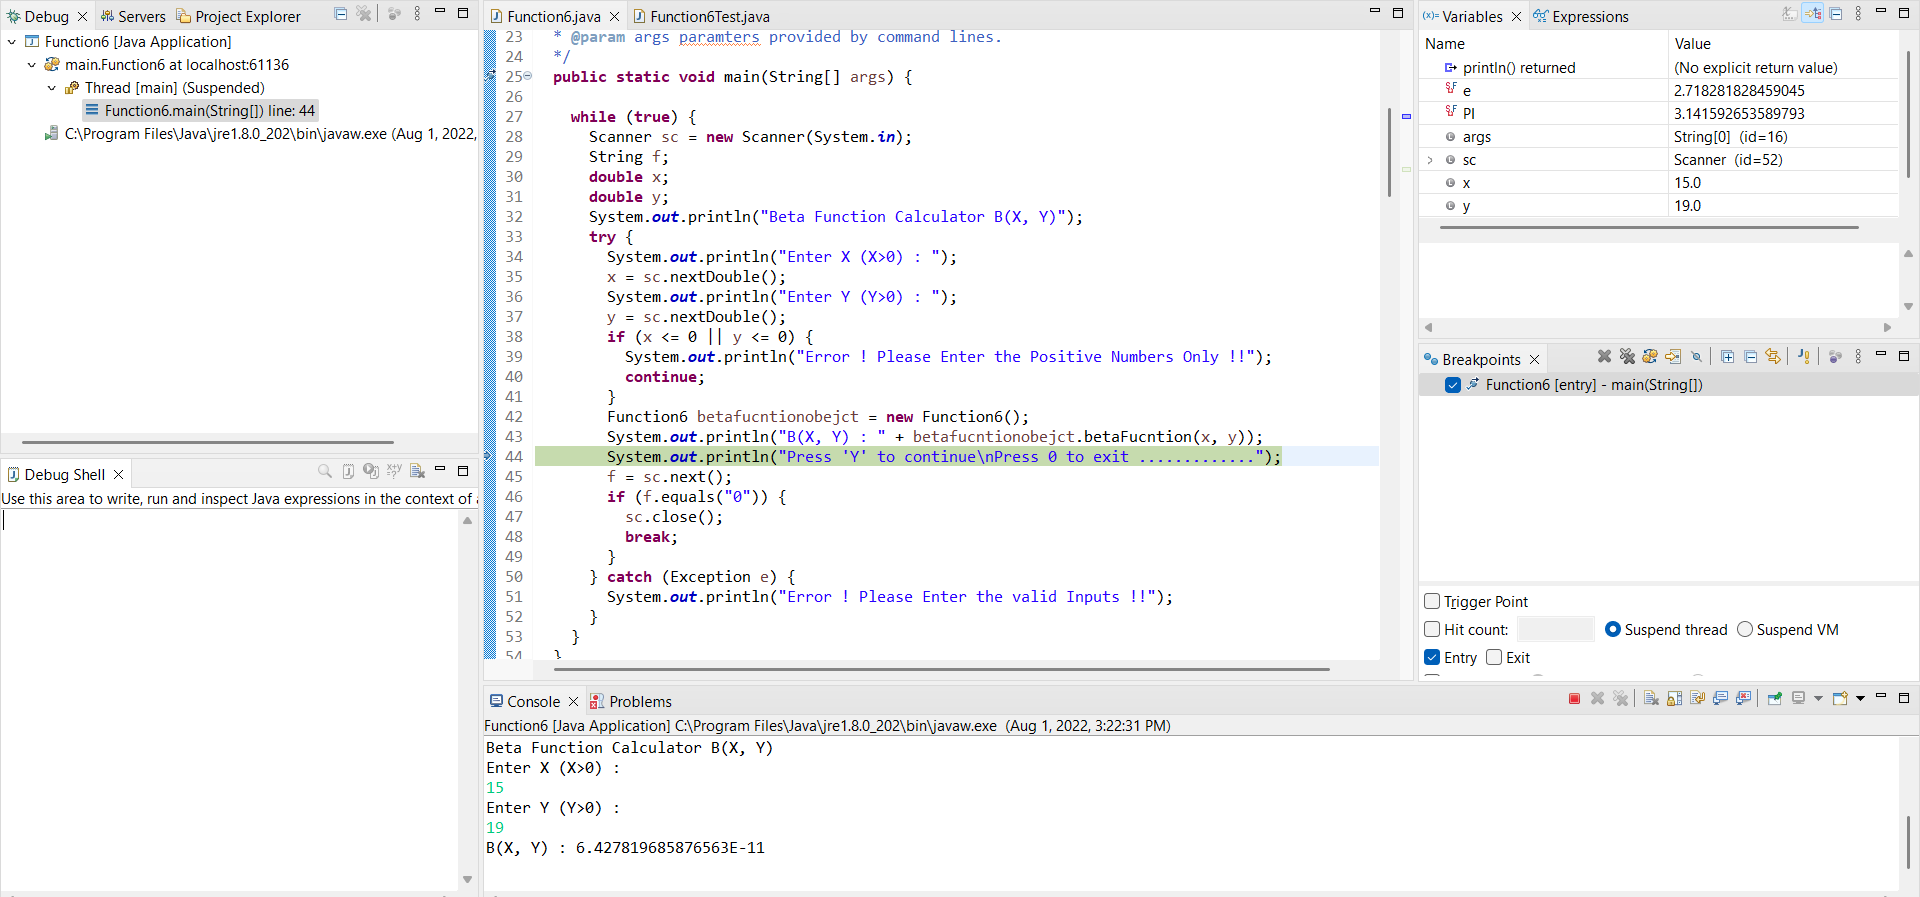
\includegraphics[width=0.73\linewidth]{Images/Debugger_snapshot.png}    
    \end{center}
    \caption{Snapshot of the Eclipse IDE debugger tool }
    \label{fig:Eclipse Debugger Tool snapshot.}
\end{figure}

\newpage
\section*{CheckStyle Tool}
The "CheckStyle" plugin for Eclipse provides the code specifications and guarantees that the java code adheres to the accepted code styles. Java code for the beta function was validated using the Google check style. Following snapshot shows there not any coding standard violations in the Beta Function code.\\
\subsubsection*{Advantages}
    \begin{itemize}[noitemsep]
        \item Supports Automatic Checking and can be used in the ongoing project. automatically checks the coding standards line by line.
        \item Supports multiple types of check styles such as Google and Sun microsystems coding standards.
        \item CheckStyle tool is portable and can be used with any IDEs and help to unify the team across various boundaries.
    \end{itemize}

\subsubsection*{Disadvantages}
    \begin{itemize}[noitemsep]
        \item To validate the coding standard, it needs to be re-compiled every time
        \item Only validate the code specification rather than apply the changes and modify them according to the given checkstyle specification.
        \item This tool has its flaws. needs to be refreshed or sometimes have to clean and build the project again to refrain from errors.
    \end{itemize}
    
\begin{figure}[h]
    \centering
    \begin{center}
    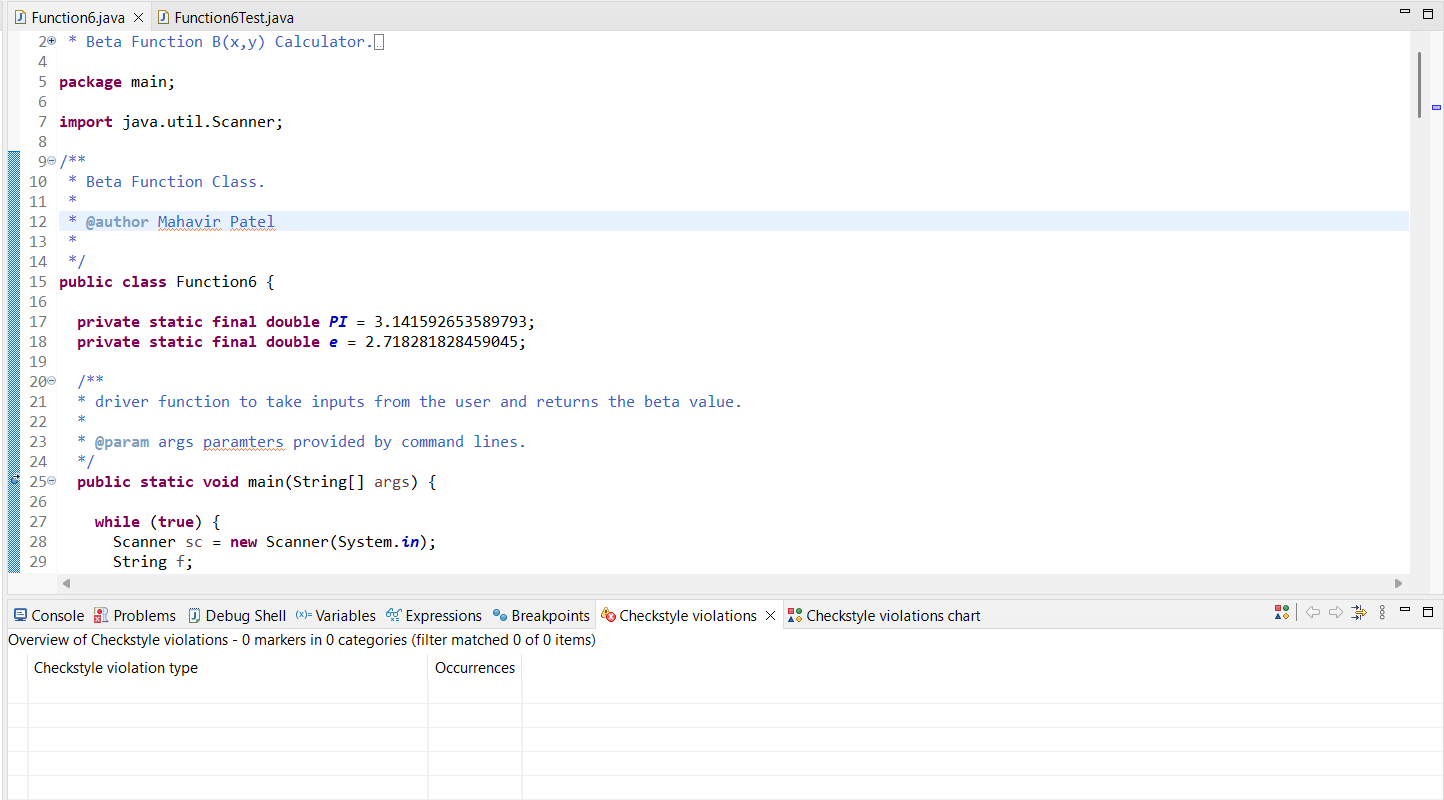
\includegraphics[width=1.0\linewidth]{Images/Checkstyle_tool_snapshot.png}    
    \end{center}
    \caption{Snapshot of the Eclipse CheckStyle plugin }
    \label{fig:Eclipse CheckStyle Plugin}
\end{figure}

\newpage
\section*{PMD - Pragmatic Quality Tool}
PMD, or programming mistake detector is a source code analyzer. It detects typical programming errors such as unnecessary variables, empty catch blocks, It detects typical programming errors such as unnecessary variables, empty catch blocks, unneccesary object creation, etc. The code error seen in the following screenshot was found in Ecplise IDE's source code and was verified using the PMD plugin. \\ 
\subsubsection*{Advantages}
    \begin{itemize}[noitemsep]
        \item By examining unnecessary variables or objects, space efficiency is increased and code analysis can be done.
        \item The copy-paste detector, or CPD, is offered. In the source code, redundant code is discovered.
        \item Multiple programming languages, markup languages, Salesforce.com Apex and Visualforce, PLSQL, Apache Velocity, XML, XSL, and other technologies are supported.
        \item Additionally PMD allows user-defined rules for source code analysis
    \end{itemize}
\subsubsection*{Disadvantages}
    \begin{itemize}[noitemsep]
        \item There are times when these programmes generate false positives and false negatives, providing the appearance that everything is being addressed.
        \item Since it is more difficult to identify the precise location of the code vulnerability, a solution takes longer to implement. Vulnerabilities in the runtime environment are not found.
    \end{itemize}

\begin{figure}[h]
    \centering
    \begin{center}
    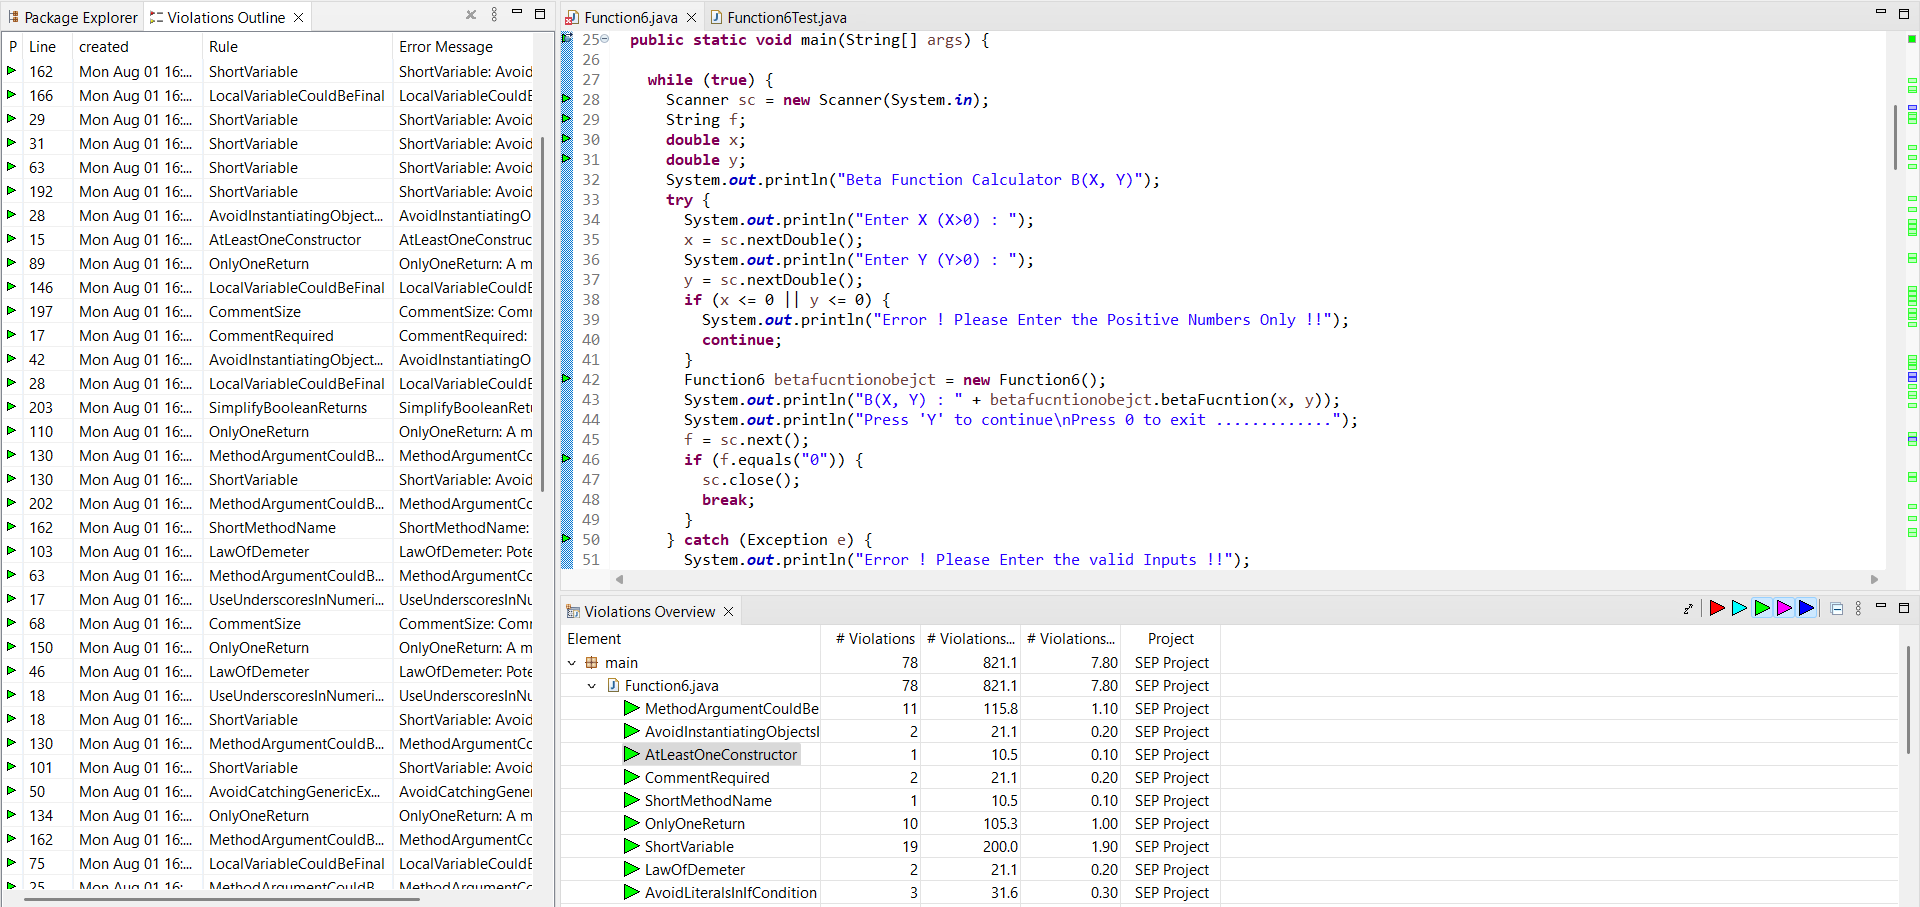
\includegraphics[width=1.0\linewidth]{Images/PMD_plugin_violations.png}    
    \end{center}
    \caption{Snapshot of the Eclipse PMD plugin}
    \label{fig:Eclipse PMD Plugin}
\end{figure}

\newpage

\section*{Quality Attributes}
\subsection*{Usability}
The beta function calculator has a straightforward user interface that is easy enough for non-technical people to understand. Additionally, it offers an error message that any user may readily understand, such as improper inputs or beta function values such as negative or zero. Even for small values of integers, the Stirlings Approximation offers the user confidence in the accuracy of the solution.
\subsection*{Maintainability}
Due to the separation of various tasks, the beta function calculator is simple to maintain without causing any system disruptions or crashes. Additionally, the user interface might be included. Furthermore, it may be adjusted to account for changes in the future and can accommodate various approaches to determine the beta values of the inputs.
\subsection*{Correctness}
The results from this calculator are correct for integer numbers. However, it delivers an accurate answer with an accuracy of up to 7 decimal places for fractional integers. Even with a small number, Stirling's approach produces almost exact results, but as the number increases, the method gives a user the right answers.
\subsection*{Efficiency}
In both space and time, the calculator application is incredibly effective. It reduces the StackOverflow error using the tail recursive method and provides correct results in a short amount of time.
\subsection*{Robustness}
The beta calculator is really reliable. It offers an error message that the user may readily understand. If invalid inputs are given, the program will continue to run without pausing the process and will give an error message based on the circumstances that led to the disruption in the flow.

\newpage
\section*{Error Message and Exception Handling}
Responding to undesirable or unexpected events that occur while a computer program is running is known as exception handling. Without this procedure, exceptions would disrupt a program's normal operation and lead to a crash. To avoid this, exception handling deals with these occurrences.\\\\
In Beta Function Calculator, if a user enters a number other than positive real numbers, then the user will be notified by an error message "Please enter the positive numbers only"\\\\
Moreover, if the user enters a String as input then the system throws an exception containing a message "Please enter the valid inputs" and for any general exception a message "Fatal error" is thrown by an exception handling mechanism.

\section*{References}
\begin{itemize}
    \item Error Handling Defination \\ \href{https://www.techtarget.com/searchsoftwarequality/definition/error-handling}{https://www.techtarget.com/searchsoftwarequality/definition/error-handling}
    \item PMD \\
    \href{https://pmd.github.io/latest/index.html}{https://pmd.github.io/latest/index.html}
    \item Debugging in the Eclipse IDE \\
    \href{eclipse.org/community/eclipse\_newsletter/2017/june/article1.php}{eclipse.org/community/eclipse\_newsletter/2017/june/article1.php}
\end{itemize}
\end{document}
